\documentclass[a4paper,10pt]{article}
\usepackage[utf8x]{inputenc}
\usepackage{array}
\usepackage{graphicx}
\usepackage{float}
\usepackage{color}
\usepackage{alltt}
\usepackage[T1]{fontenc}
\usepackage{ae,aecompl}
\usepackage{natbib}
\usepackage{url}

\bibpunct{[}{]}{;}{a}{}{,}

%opening
\title{General Context-Free Top Down Parsing in Cubic Time}
\author{Arnold Lankamp}

\begin{document}

\maketitle

\pagebreak
\begin{abstract}

In this article we will describe our general top-down parsing algorithm. The intent of this algorithm is to be both easy to comprehend and able to perform well on any grammar. In our opinion users should not be required to refactor their grammars to enable the parser to complete within an acceptable amount of time. Nor should it be difficult to comprehend what is going on under the hood, enabling one to easily visualize what is going on. From a developer's point of view, creating an implementation of the algorithm should also be similarly easy to do; often this is something that requires a considerable amount of effort to get right. While this sounds fairly ambitious, we managed it. We created a general parsing algorithm that is both easy to understand and can compete with any other general parsing algorithm out there in terms of scalability and performance.

\end{abstract}

\section{Introduction}

For our parsing algorithm we choose for a top-down approach, as it is more in-line with human thinking then bottom-up. This makes both the algorithm and implementation(s) easier to comprehend and makes parse traces easier to visualize. Top-down parsers also have no need for complicated parse tables; the translation from a grammar to a for the parser usable format can simply be one-on-one, without any additional trickery or risks of parse table explosion. Lastly, top-down parsers can also generate understandable error reports more easily, which is a very welcome feature. We call our parser, the Scannerless General Top Down Binary Forest Parser or SGTDBF.

To give an impression of the capabilities of our algorithm and implementation, we will enumerate some highlights first:
\begin{itemize}
 \setlength{\itemsep}{0pt}
 \setlength{\parskip}{0pt}
 \setlength{\parsep}{0pt}
 
 \item Worst-case cubic time and space bounds with respect to the length of the input.
 \item Worst-case quadratic performance on unambiguous grammars.
 \item Deterministic on all classes of LL and LR\cite{knuth1965translation} grammars.
 \item No penalty for handling nullables, hidden recursive or otherwise.
 \item No penalty for being scannerless.
 \item Generating or hand crafting the parse table / code from a grammar is trivial.
 \item Parse traces are easy to visualize.
 \item Can be implemented either as breadth-first or recursive decent.
 \item Native EBNF support.
 \item Extensive build-in disambiguation features.
\end{itemize}

\pagebreak
\section{Recognizer}

First we will discuss the algorithm for the recognizer, for simplicity's sake. Further on in this article we will explain how the recognizer can be extended to become a parser.

Different variations of the algorithm are possible and while the recursive decent variant of the algorithm is more `beautiful', the main focus of this article will be on the breadth-first version of the algorithm. The reason for this is that it is the more complicated of the two, deserving of more attention and also likely the one people will end up using because of its efficiency. See section \ref{sec:breadthFirstVsDepthFirst} for more details about this.

\subsection{Graph}

To represent the parallel stacks we use a directed cyclic graph; inspired by GLR's Graph Structured Stack. While it serves a similar purpose, the way it is used is completely different. Simply put, while GLR parsers store their `history' in the GSS\cite{tomita1985efficient}, we use it to model possible `futures'.

Each graph node consists of an item, edges back to their `parents' in the graph, information about its `right neighbour' in the production, the location in the input string it is associated with and a unique identifier. Each stack node is unique for each identifier, location combination. The identifiers for the graph nodes are assigned in the following way. If we take the grammar: $S\,::=\,AB\,|\,BA,\,A\,::=\,a,\,B\,::=\,b$, this is how these identifiers could be distributed: $.S$(-1), $.AB$(0), $A.B$(1), $.BA$(2), $B.A$(3), $.a$(4) and $.b$(5). The reason these identifiers are needed is because we require them to handle the sharing of graph nodes correctly; so regardless whether or not comparable items exist, they should not be assigned the same identifier.

\subsection{The basic principle}

The basic idea behind the algorithm is fairly straightforward. In general terms this is how it works:

\begin{enumerate}
 \setlength{\itemsep}{0pt}
 \setlength{\parskip}{0pt}
 \setlength{\parsep}{0pt}

 \item Expand the left most node of every production that did not match anything yet on all stacks, until there are no stacks can be expanded anymore (i.e. they all have a terminal at the bottom).
 \item Match all nodes on the bottom of the stacks to the input. Queue the ones that match for handling and discard the ones that do not.
 \item For each node that needs to be handled, either execute a `reduce' action, queueing their parent(s) for handling (in case the node was the last in the production) or execute a `move' action, queueing the `next' node in the production they are a part of for expansion. Repeat this process until there are no nodes left to handle.
 \item If there are nodes queued for expansion go to 1.
 \item If the end of the input has been reached and we have at least one derivation for one of the start symbols and are successful; otherwise recognition failed.
\end{enumerate}

\pagebreak
\subsection{Pseudo-code}

In this section we will present and discuss the pseudo-code of the recognizer. Note however that this pseudo-code already contains the edge related optimizations listed in section \ref{sec:edgeOptimizations}. This was done since, besides improving performance, they simplify the implementation of the algorithm slightly and they enable the recognizer to achieve most of its advertised performance guarantees. We will not go into detail about how these optimization work or why they are correct here; please refer to the indicated section for more details. Other optimizations were not merged in with the code presented here, since they either complicate things too much or can be implemented in multiple ways; a decision we would like to leave for the implementer. For the same reason, the hidden right recursion fix, discussed in section \ref{subsec:hiddenRightRecursion}, was left out here as well. On the other hand, the nullable fix described in section \ref{subsec:nullables} is present.

\subsubsection{Main}
{\small
\begin{verbatim}
main(){
  toExpandSet.add('startNode');
  expand();
  
  while(hasMoreStacksToReduce(toReduceStore)){
    expandedSet.clear();
    reducedStore.clear();
    sharedNextSet.clear();
    toReduceSet = getStacksToReduce(toReduceStore);
    
    do{
       reduce();
       expand();
    }while(isNotEmpty(toReduceSet));
  }
  
  if(endOfInputHasNotBeenReached()) error;
}
\end{verbatim}
}

This is the main function of the recognizer. It starts with building the stacks for the first level, by queueing the `start node' and expanding it. Once it has done so it will keep alternating between reducing and expanding until there are no more stacks left alive. At the start of each iteration we get the appropriate {\bf toReduceSet} from the {\bf toReduceStore}. The {\bf toReduceStore} is a collection that contains one {\bf toReduceSet} for each level. At the end of each iteration we check whether or not we need another iteration in the current level or need to shift to the next one. In case we shifted we need to discard all level specific data. This retention of data between iterations in the other case is necessary to be able to handle nullables properly. For more information about the handling of nullables see section \ref{subsec:nullables}.

Note that the {\bf toReduceStore} needs to be implemented as an array or table with O(1) look-up time; otherwise it is not possible to guarantee worst-case cubic time complexity.

Also note that after each iteration all graph nodes that are no longer reachable through any of the nodes in the {\bf toReduceStore}, can be discarded.

\pagebreak
\subsubsection{Expansion}
\label{subsec:pseudocodeExpand}
{\small
\begin{verbatim}
expand(){
  while(node <- toExpandSet){
    if(node.isTerminalOrEpsilon()){
      if(node.match(input)){
        toReduceStore.add(node);
      }
    }else{
      if(cachedEdges.contains(node.sort)){
        edgesSet = cachedEdgesMap.get(node.sort);
      }else{
        edgesSet = createAndCacheEdgesSet(node.sort);
        
        for(childNode <- getAlternatives(node)){
          childNode = childNode.initialize(location);
          childNode.setEdgesSet(edgesSet);
          toExpandSet.add(childNode);
        }
      }
      edgesSet.addEdge(node);
      
      if(reducedStore.contains(node.sort)){
        toReduceSet.add(node);
      }
    }
  }
}
\end{verbatim}
}

This is the expand loop. It will iterate over the {\bf toExpandSet} until there are no more stacks queued for expansion. While expanding we check the type of the node we are handling. If the node is a terminal or an epsilon it needs to match the input (epsilons naturally always match). If it matches, it is added to appropriate {\bf toReduceSet} in the {\bf toReduceStore}; otherwise we discard it, causing the stack it was associated with to die of. If the node is associated with a non-terminal, we check if there is a cached set of edges available for that non-terminal's sort. If there is, we queued the alternatives for that non-terminal sort before; since this is the case, we merge the current stack with the already expanded ones by adding an edge to the cached {\bf edgesSet} for this non-terminal sort. If a cached {\bf edgesSet} is not available, we have not encountered a non-terminal of this sort yet and need to expand it. We do this by retrieving its alternatives and queueing the first `child' of each alternative for expansion, by adding them to the {\bf toExpandSet}. We also create and cache a set of edges for this non-terminal sort, to which an edge to the current node will be added. Each of the `child' nodes will receive a reference to this {\bf edgesSet}, which may be updated with additional edges later on in the expansion process.

Finally we check whether or not there have been nullable reductions for the non-terminal sort associated with the current node. This can occur because we to multiple iterations in this same level to be able to handle nullables properly. If such a nullable reduction is present in the {\bf reducedStore}, we queue the current node for reduction by adding it to the {\bf toReduceSet} for the current level. We will discuss the handling of nullables in more detail in section \ref{subsec:nullables}.

\pagebreak
\subsubsection{Reduction and moving}
{\small
\begin{verbatim}
reduceAndMove(){
  while(node <- toReduceSet){
    if(node.lastInProduction()){
      for(edgeLevel <- node.edgesPerLevel){
        sort = edgeLevel.getOne().sort;
        if(reducedStore.notContains(sort)){
          reducedStore.add(sort);
          
          for(edges <- edgeLevel){
            toReduceSet.add(parent);
          }
        }
      }
    }else if(node.hasNext()){
      next = node.next.initialize(location);
      
      if(sharedNextSet.contains(next)){ // Sharing
        next = sharedNextSet.get(next);
      }else{
        sharedNextSet.add(next);
        toExpandSet.add(next);
      }
      next.addEdges(node.edges);
    }
  }
}
\end{verbatim}
}

This is the reduce and move loop. It will iterate over the {\bf toReduceSet} until there are no more stack nodes queued for reduction. When a node is being reduced, one of two things can happen. Either it is the last node in the production and we need to queue the `parents' of this node for reduction (if not reduced of queued for reduction already), by adding them to the {\bf toReduceSet}. Otherwise we need to move to the `next' node in the production, queue this `next' node for expansion and transfer all edges from this node to it. If the `next' node has already been scheduled for expansion it will be present in the {\bf sharedNextSet}. If this is the case we need to retrieve the shared equivalent of this `next' node from this set and add the edges to that node instead.

The edges are grouped by level. This level indicates the start location of the node the edge points to. To check whether or not the parents of a node need to be queued for reduction, we get one of the edges from each {\bf edgeLevel} and check if there are reductions for the non-terminal sort associated with the node this edge points to, by consulting the {\bf reducedStore}. If a node has not been reduced yet, we queue all of the nodes that are pointed to from edges in that {\bf edgeLevel} for reduction; otherwise we do not. This will work correctly since every node containing a non-terminal of the same sort always has exactly the same alternatives in the same level. Note that this behaviour is not a necessity, but an optimization (which, potentially, reduces the number of edge visits by a factor between one and the number of non-terminals in the grammar). For more information about this optimization see section \ref{subsec:edgeVisitOptimization}.

The {\bf reducedStore} is a dual layered data structure. The first layer is indexed by the {\bf start location} of the node and the second layer by the sort of the non-terminal in the node. For each level the {\bf reducedStore} can contain a variant for every non-terminal for each possible substring up until the current location. This {\bf reducedStore} is necessary to keep track of which nodes have been reduced yet. The first layer of the {\bf reducedStore} needs to be implemented as an array or table with O(1) look-up time; otherwise it is not possible to guarantee worst-case cubic time complexity.

\subsection{Correctness}

In this section we will go into detail on some special cases that deserve some additional attention.

\subsubsection{Left recursion}
First of all, left recursion. Normal top-down parsers cannot handle grammars containing left recursion, since they keep expanding left recursive rules indefinitely, preventing implementations of these kind algorithms from terminating. Because we introduce sharing into the graph, which leads to automatic terminalization of all these rules, this undesirable behaviour is prevented from manifesting. By terminalization we mean that the expansion phase converges to a point at which each stack has a terminal at the bottom and thus cannot be expanded further. For example, if we take the grammar:\\
$S ::= A$\\
$A ::= Aa\,|\,a$\\
We would expand these rules in the following way:
\begin{figure}[H]
\centering
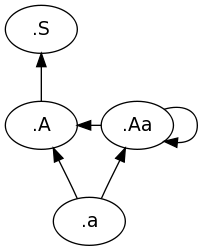
\includegraphics[scale=0.5]{left-recursive.png}
\caption{A graph representation after the initial expansion phase of a left-recursive grammar.}
\end{figure}
As can be seen a cycle is added to the graph, since $.Aa$ is, in a way, a child of itself. To see how left recursive grammars work in action see section \ref{sec:tracesLeftRecusive}.

\subsubsection{Cycles}
Cycles present another issue that needs to be handled. Similarly to left recursion, this problem is automatically resolved by the sharing that is introduced into the graph. Instead of infinitely expanding circularly dependent production rules, a cycle will be added to the graph, halting the expansion process for the involved rule. The reduction process will also terminate, since the recognizer only performs the reductions for each node once.

\subsubsection{Nullables}
\label{subsec:nullables}
Nullables also deserve some attention. Nullables do not pose any difficulties in most cases; however when a node that is associated with a nullable non-terminal gets queued for expansion in two or more separate iterations in the same level, which can happen when a production contains two or more identical consecutive nullables for example, problems arise. The first of these problems is sharing related.

We will describe the issue by illustrating what would happen in a version of the implementation of the algorithm which does not contain the fix.
Consider the following grammar:\\
$S ::= AA$\\
$A ::= B$\\
$B ::= \epsilon$\\
Input = <empty>\\
After the first expansion and reduction phase, we matched both $.B$ and the $.AA$ at location $0$. Next we move to $A.A$; when we expand the $A.A$ node we notice $.B$ has already been expanded at the current level ($0$), causing recognition to stop. Since there is no work left to do, the recognizer will terminate with an error, as we failed to produce any derivations for the input string.

In our algorithm we address this issue by checking whether or not the non-terminal associated with the node we are currently attempting to expand has nullable results in the current level. If this is the case we queue this node for reduction. Additionally, we also update the appropriate set of edges (as described in section \ref{subsec:pseudocodeExpand}). This is necessary, since the children of the current node were already expanded in a previous iteration in the same level; this means the current stack needs to merge with the stacks of these children, so no future (non-nullable) reductions involving these children will go missing. We will keep alternating between expansion and reduction until no more work can be done for the current level (i.e. there are no more nullable reductions); once this is the case, we shift to the next level.

\subsubsection{Hidden right recursion}
\label{subsec:hiddenRightRecursion}
Unfortunately solution described above only solves one of the two nullable related problems. The other issue that needs to be resolved is related to hidden right recursion.

Consider the following grammar:\\
$S\,::=\,SS\,|\,a\,|\,\epsilon$\\
Input = $a$\\
Imagine we matched the some part of the tree and are at level $1$ now. We are trying to recognize $.SS$ and $S.S$, where $S.S$ has a prefix that starts at $0$. This means $.SS$ only has edges that point to nodes in level $1$ and $S.S$ only has edges that point to nodes in level $0$. The problem is that the order in which we handle these two nodes will determine whether or not we recognize all derivations. If we would move from $S.S$ to $SS.$ first, $SS.$ will only have edges to level $0$ associated with it, so this will cause us to miss the reductions to level $1$ when $SS.$ is handled. This happens because the stack merge at $S.S$ took place after $S.S$ was handled, preventing the edges present on $.SS$ from being transferred, through $S.S$, to $SS.$. On the other hand, if we would move from $.SS$ to $S.S$ first, the stacks would merge before $S.S$ gets handled. In this case $S.S$ would contain edges to both the nodes in level $0$ as the ones in $1$ before we move to $SS.$, which does lead to a correct result.

This order dependency is something we cannot enforce, so we need another solution for this problem. We solved this by propagating edges forward through the production, when necessary. If we are currently handling a node associated with nullable derivations and are moving to the next node in the production, we need to check whether or not this next node is handled yet and if it is associated with nullable derivations as well. If this next node is both handled and has nullable derivations associated with it, we transfer all edges that are absent on this next node to it. If missing edges were transferred, we need to continue the propagation of specifically these transferred edges to the node beyond this next node and so on until the last node in the production is reached. For each edge that is transferred to the last node in the production a reduction needs to be performed. This way we can be sure all derivations will be traversed.

Also note that, since this propagation only happens within a single level and does not introduce any real extra work, it does not influence worst-case behaviour. This is because all stack merges would have happened regardless of their timing. The only difference is that the exact same amount of work they normally generate gets distributed over multiple visits of the same node. Consequently, the performance impact of this solution is very low in general; close to non-existent even, since it only requires one cheap constant time check on each node visit. See section \ref{sec:worstcaseBench} for related benchmark results.

\subsubsection{Termination}
Another questions that some people will have on their mind is: ``does it terminate?". Of course it does. The reason for this fairly obvious and can be even explained in one sentence; since we move forward to the next level once all work is done in the current level and we share all graph nodes within each level (of which there are a finite amount), causing the expansion and reduction phases to converge to a point where no more work can be done in a level, we are always able to reach the end of the input string (assuming the input string has a finite length), completing recognition.

\subsection{Breadth-first vs depth-first}
\label{sec:breadthFirstVsDepthFirst}

While we focussed on a level synchronized version of our algorithm, it also possible to implement a recursive decent variant.

The main difference with a recursive decent approach is that we can now have (non-nullable) stacks running ahead of others. To ensure we register all derivations, we need to apply a solution that is almost identical to the hidden right recursion fix, which we discussed in section \ref{subsec:hiddenRightRecursion}. When a stack merge occurs we need to propagate the edge associated with the node we are currently handling forward, towards the end of all possible continuations of the production that we already recorded and execute the proper reductions in case this edge is not present yet on the node that is associated with a final item in the production. Naturally, we can halt the propagation for a path as soon as we detect that the edge we intended to add is already present; if we would not do this the amount of node visits would become unbound polynomial in the worst-case.

Note however that while the absolute amount of `work' required by the algorithm does not increase, the worst-case amount of node visits increases from $O(N)$ to $O(N^2)$, however the number of edges that is merged in during each visit is always $1$, instead of $N$ in the worst-case. Because of this the worst-case behaviour (section \ref{subsec:recognizerComplexity}) is not influenced by this. Nor will it have an effect on the time bound for unambiguous grammars (section \ref{subsec:unambiguousTimeComplexity}).

Conceptually the recursive decent version looks nicer, since there is no real distinction between normal control flow and the handling of nullables. On the other hand, the implementation for the recursive decent variant requires extra bookkeeping, as it basically implements backtracking in combination with memoization and thus needs information about all levels, instead of just the current one. For similar reasons, it will never be as efficient as a level synchronized variant, both in terms of performance as memory usage. However, since it may be desirable to create a recursive decent implementation in certain cases, we offer both options to the user / implementer, so they are able to make their own decision.

\subsection{From grammar to recognizer}

Converting a grammar into a format the recognizer or parser can use, either by hand or by generating it, is relatively straight forward. All that is needed is a direct translation from the grammar rules to either functions or a table like data structure. Basically the recognizer just needs to know what alternatives are associated with each left-hand-side. For example, in case one generates code, this means there would need to be one function per non-terminal sort, which contains logic that informs the recognizer about what alternatives to expect.

Since the mapping between the original grammar and the code or table is one-on-one, it is possible to write or edit it by hand without much effort. In fact hand crafting it is about as simple as writing the grammar itself (although more cumbersome).

Another advantage is that, in combination with the top-down-ness of our algorithm, it makes tracing errors in a grammar easier; if you would like to know why something did not match at a certain position, you can just go through it with a debugger to see what happens. Your degree of success naturally depends on the amount of stacks that are alive at the moment you are trying to observe, which is linked to the amount of non-determinism in the grammar, but at least the possibility to do so exists.

\subsection{Example traces}

To illustrate how the recognizer works in action, we constructed some example traces using various grammars to give an impression.

\pagebreak
\subsubsection{Straight forward}
First we will take a look at a simple non-ambiguous grammar:\\
$S ::= AB$\\
$A ::= a$\\
$B ::= b$\\
Input = $ab$

\begin{enumerate}
 \setlength{\itemsep}{0pt}
 \setlength{\parskip}{0pt}
 \setlength{\parsep}{0pt}
 
 \item expand $.S$
 \item expect $.AB$
 \item expand $.AB$
 \item expect $.a$; $.a$ matches
 \item reduce $a.$ and follow edge to $.AB$
 \item move from $.AB$ to $A.B$
 \item expand $A.B$
 \item expect $.b$, $.b$ matches
 \item reduce $b.$ follow edge to $A.B$
 \item reduce $AB.$ and follow edge to $.S$
 \item parse for $S.$ is complete 
\end{enumerate}
This one is easy to follow and does not really need any additional explanation.

\subsubsection{Left recursive}
\label{sec:tracesLeftRecusive}
Next up is a grammar containing a left-recursive rule:\\
$S ::= A$\\
$A ::= Aa\,|\,a$\\
Input = $aaa$

\begin{enumerate}
 \setlength{\itemsep}{0pt}
 \setlength{\parskip}{0pt}
 \setlength{\parsep}{0pt}
 
 \item expand $.S$
 \item expect $.A$
 \item expand $.A$
 \item expect $.Aa$ and $.a$; $.a$ matches
 \item expand $.Aa$ $\Rightarrow$ $.Aa$ shared
 \item reduce $a.$ and follow edges to $.A$ and $.Aa$
 \item reduce $A.$ and follow edges to $.S$
 \item parse for $S.$ is incomplete and is discarded
 \item move from $.Aa$ to $A.a$; $A.a$ matches
 \item reduce $Aa.$ and follow edges to $.A$ and $.Aa$
 \item reduce $A.$ and follow edges to $.S$
 \item parse for $S.$ is incomplete and is discarded
 \item move from $.Aa$ to $A.a$; $A.a$ matches
 \item reduce $Aa.$ and follow edges to $.A$ and $.Aa$
 \item reduce $A.$ and follow edges to $.S$
 \item parse for $S.$ is complete
 \item move from $.Aa$ to $A.a$; $A.a$ does not match since the EOI has already been reached
\end{enumerate}
As one can see, when expanding $.Aa$ (at 5), sharing is detected causing a cycle to be added to the graph. Reductions of $Aa.$ follow the edge back to $.Aa$ which will move to $A.a$; this will lead to one $a$ being matched at each `iteration' and ultimately consuming all of them.

\subsection{Worst-case time complexity}
\label{subsec:recognizerComplexity}

We are designing a parsing algorithm that is intended to scale as well as is possible, regardless of the input grammar. For this reason, the recognizer must not break the cubic time bound. Here we will prove that we remain within this bound.

Reducing consumes $O(N^3)$ time in the worst-case; where $N$ is the number of characters in the input string. Every edge is associated with one reduction per level per graph node at most. Each of these edges can be associated with $O(N)$ nodes per level; one per level before the current level. There are $N$ levels, so each edge will be visited $O(N^2)$ times at most. Since there are never more then $O(N)$ edges in total, we can conclude that the number of visited edges falls within the $O(N^3)$ bound. Each of the operations executed during an edge visit completes in constant time, so the worst-case time bound of the reducer is directly related to the number of edge visits.

As for stack merges, since the graph only contains nodes for non-terminal sorts that we expect to encounter, there are at most $O(N)$ of them. Each graph node only has one edge to each of its possible parents per level and there are $N$ levels, so there are at most $O(N)$ edges per node. In the worst-case there are $N$ nodes that match a substring that ends at the current level. When moving to the next node in the production, all edges of these nodes need to be carried over. Since these sets of edges need to be merged, the time this operation needs to complete is equal to the number of levels before (and including) the current level (so $N$ at most). So the time required to execute stack merges remains within $O(N^2)$ in the worst-case.

Overall, this means that the algorithm remains within cubic time bounds in worst-case scenarios.

\subsection{Time complexity for unambiguous cases}
\label{subsec:unambiguousTimeComplexity}

Keeping worst-case behaviour in check is great, but is generally of lesser importance then having good performance and scalability in the more common cases. Here we will discuss the performance of our algorithm on unambiguous context-free grammars.

Lets first specify how the usage of an unambiguous grammar limits the behaviour the recognizer exhibits. Ambiguities only arise when stacks split into two or more alternative paths and recombine back into one; this indicates that a part of the input can be validly interpreted in more then one way. For unambiguous grammars this behaviour never occurs. While it is still possible for stacks to split, just as it is possible for stacks to merge, no combination of any of these splits and merges can ever be related.

Using splits and merges as behavioural indicators, we can categorize unambiguous grammars in different classes and give specific performance guarantees for each of them.

First of all we have deterministic grammars. For these types of grammars we can guarantee linear performance, since there will never be more then one live stack during recognition. In our case, all classes of LL and LR grammars fall in this group. Note however that prefix sharing (see section \ref{sec:prefixSharing}) is required to enable deterministic behaviour for LR grammars, although we can guarantee never to break the linear time bound regardless of this.

Additionally there are unambiguous grammars for which stacks can split, but never merge. We can also guarantee linear performance on these. The reason for this is that, while there can be more then one live stack at any given point, each node in the graph will never have more then one edge, because stack merges never occur. Note however that, while the time bound for these types of grammars is guaranteed to be $O(N)$, performance will degrade relative to the amount of non-determinism. Certain grammars containing left recursive rules, for example, fall in this group.

Finally, we also have unambiguous grammars for which both stack splits and merges occur. This group represents the worst-case, which has a $O(N^2)$ time bound. Because stacks can merge in these cases, each graph node could potentially have edges to $N$ different levels. Which means there can be $N$ reductions per node at most, instead of just $1$. Grammars containing rules like $S ::= aSa\,|\,a$, for example, fall in this group.

However, we would like to point out that the performance of the recognizer is directly linked to the amount of non-determinism in the grammar; indicating that performance degradation should be fairly graceful, also for ambiguous grammars. This means that recognizing input strings for near deterministic grammars will also complete in near linear time. Our assumption is that deterministic or near-deterministic grammars represent the majority of real grammars. Regardless of this, our performance guarantees are at least as good as those of any other general recognizer algorithm.

\subsection{Error reporting}

We would also like to note the relative ease with which understandable error reports can be generated. When a parse error is encountered it is trivial to generate all possible traces back to the root from the current level, since we have all the necessary information present in the graph. In these traces a user can exactly see where recognition failed, but also what did match up until this point.

\section{Parser}

\subsection{Parse forest}

To represent the parse forest we use a format that was specifically designed for this parser, to ensure worst-case behaviour remains within cubic space and time bounds. We will simply refer to this type of parse forest as being binarized, for lack of a proper name. While its purpose is similar to binarized SPPFs\cite{scott2007brnglr}, its implementation is different.

The parse forest consists of nodes. Every node in the forest contains a result and a set of prefixes. Each result represents a substring for a certain symbol. In case this symbol is a non-terminal sort, this result contains one or more references to alternative representations of the substring it denotes. If the symbol is a terminal, it will just represent that specific terminal. The set of prefixes contained in the node hold all possible alternatives for the preceding item in the production. (Naturally this set is empty for the node associated with the first item in the production). A prefix only consists of a reference to a node. If one traces all possible paths through this representation of a production to the start, one will get all alternatives for this production of the substring it represents.

Note however that there is a strong relation between the internal graph representation of the parser and the resulting parse forest. Because of this relation, the resulting parse forest can contain cycles.

Another thing worth mentioning is that it is not strictly required to use a binarized parse forest in combination with our parser. In reality any kind of representation could be used, though it is highly recommended to use the one described here for optimal performance and ease of implementation. For more discussion about the cubic vs non-cubic parse forest trade-off see section \ref{subsec:Binarization}.

\subsubsection{Example}
To give an idea of what a typical parse forest would look like we will give a simple example using the following grammar:\\
$S\,::=\,AAA$\\
$A\,::=\,a\,|\,aa$\\
Input = $aaaa$

\begin{figure}[H]
\centering
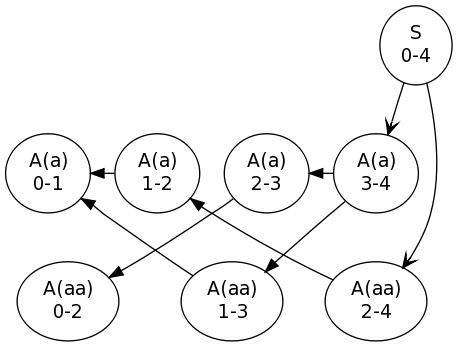
\includegraphics[width=0.5\textwidth]{a_aa-forest.png}
\caption{A visual representation of the parse forest, showing all derivations for the given input string. The numbers indicate the start and end position of the matched substring.}
\end{figure}

In the figure above we see the parse forest. It illustrates how the parse results are stored in memory.

To show how we can obtain all possible derivations from this parse forest, we will list them in the table below; which relates each path through the forest to a derivation.

\begin{table}[H]
\centering
\begin{tabular}{ p{15em} p{15em} }
Derivation & Forest path\\
\hline
S(A(a),A(a),A(aa)) & $A0$-$1$ $\leftarrow$ $A1$-$2$ $\leftarrow$ $A2$-$4$\\
S(A(a),A(aa),A(a)) & $A0$-$1$ $\leftarrow$ $A1$-$3$ $\leftarrow$ $A3$-$4$\\
S(A(aa),A(a),A(a)) & $A0$-$2$ $\leftarrow$ $A2$-$3$ $\leftarrow$ $A3$-$4$
\end{tabular}
\caption{A flattened representation of the parse forest, listing all derivations.}
\end{table}

\pagebreak
\subsection{Pseudo-code}

Augmenting our recognizer with parse tree construction code is trivial. Only a few minor adjustments are needed. Relevant pieces of code, containing changes or additions, are highlighted in italics.

\subsubsection{Main}
{\small
\begin{alltt}
main()\{
  toExpandSet.add('startNode');
  expand();
  
  while(hasMoreStacksToReduce())\{
    expandedSet.clear();
    resultStore.clear();
    sharedNextSet.clear();
    toReduceSet = getStacksToReduce();
    
    do\{
       reduce();
       expand();
    \}while(isNotEmpty(toReduceSet));
  \}
  
  if(endOfInputHasNotBeenReached()) error;
  \textit{
  return resultStore.get('startNode');}
\}
\end{alltt}
}

The only things that need to be changed in the main function to transform the recognizer into a parser are the returning of the final result (if not in error) and replacing the {\bf reducedStore} by {\bf resultStore}. The {\bf resultStore} is similar to the {\bf reducedStore}, except that it also contains the result associated with the non-terminal sorts in the store.

Note that, like the {\bf reducedStore}, the {\bf resultStore} is a dual layered data structure. The first layer is indexed by the {\bf start location} of the result and the second layer by the sort of a non-terminal. In each level the {\bf resultStore} can contain a variant for every non-terminal for each possible substring up until the current location. The first layer of the {\bf resultStore} needs to be implemented as an array or table with O(1) look-up time; otherwise it is not possible to guarantee worst-case cubic time complexity.

\pagebreak
\subsubsection{Expansion}
{\small
\begin{alltt}
expand()\{
  while(node <- toExpandSet)\{
    if(node.isTerminalOrEpsilon())\{
      if(node.match(input))\{
        toReduceStore.add(node);
      \}
    \}else\{
      if(cachedEdges.contains(node.sort))\{
        edgesSet = cachedEdgesMap.get(node.sort);
      \}else\{
        edgesSet = createAndCacheEdgesSet(node.sort);
        
        for(childNode <- getAlternatives(node))\{
          childNode = childNode.initialize(location);
          childNode.setEdgesSet(edgesSet);
          toExpandSet.add(childNode);
        \}
      \}
      edgesSet.addEdge(node);
      \textit{
      if(resultStore.contains(node.sort))\{}
        toReduceSet.add(node);
      \}
    \}
  \}
\}
\end{alltt}
}

The expansion code does not need to change a lot either, since it has limited interaction with parse results. The only change is related to the {\bf reducedStore}, which has been replaced by the {\bf resultStore}. In this context the {\bf resultStore} serves a similar function as the {\bf reducedStore} in the recognizer; to check whether or not there are nullable reductions available for a certain non-terminal sort. We will discuss the {\bf resultStore} in more detail further on in this section.

\pagebreak
\subsubsection{Reduction and moving}
{\small
\begin{alltt}
reduceAndMove()\{
  while(node <- toReduceSet)\{
    if(node.lastInProduction())\{
      for(edgesLevel <- node.edgesPerLevel)\{\textit{
        if(resultStore.contains(edgesLevel.getOne().sort))\{
          result = resultStore.get(edgesLevel.getOne().sort);
        \}else\{
          result = createResult(edgesLevel.getOne());}
          for(edges <- edgesLevel)\{
            toReduceSet.add(parent);
          \}
        \}\textit{
        result.addAlternative(node.prefixes, node.results);}
      \}
    \}else if(node.hasNext())\{
      next = node.next.initialize(location);
      
      if(sharedNextSet.contains(next))\{ // Sharing
        next = sharedNextSet.get(next);
      \}else\{
        sharedNextSet.add(next);
        toExpandSet.add(next);
      \}
      next.addEdges(node.edges);\textit{
      next.updatePrefixes(node.prefixes, resultStore.get(node));}
    \}
  \}
\}
\end{alltt}
}

The reduce and move code needs to be modified more extensively. Basically two things need to be added.

First of all the storing of results. We need to create (at most) one {\bf result} per sort of non-terminal for each matched substring. In the recognizer code we used the {\bf reducedStore} for a similar purpose. Here it is replaced by the {\bf resultStore}, which is basically the same thing, but instead it associates results with non-terminal sorts.

Secondly we need to add {\bf prefixes} to the nodes that are being queued for expansion when we are moving to the {\bf next} node in the production. We do this by creating a new prefix using the prefix of the current node and its result and adding it to the {\bf next} node. We add the prefixes to graph nodes for convenience reasons; regardless of where the result(s) of the node end, they will always share the same prefix. By adding the prefixes to the graph nodes they are easy to retrieve; all these nodes need is a collection that holds all the prefixes for it, grouped by the start location of the production each individual node is a part of.

\pagebreak
\subsubsection{Results}
{\small
\begin{alltt}
\textit{createResult(node)\{
  result = allocateResult(node.startLocation, node.sort);
  resultStore.add(result);
  return result;
\}}
\end{alltt}
}

We also need a function for creating results. Every time a {\bf result} is created we need to add it to the {\bf resultStore}. The {\bf start location} and non-terminal {\bf sort} of the given node are used as keys. Like the {\bf reducedStore} the {\bf resultStore} is a dual layered data structure, where the first layer is indexed using the {\bf start location} of the node and the second layer by the non-terminal {\bf sort} the node represents.

\subsection{Correctness}
\label{sec:parserCorrectness}

Since the conversion of our recognizer to a parser is so trivial, the parser is as correct as the recognizer. The only thing that may require some additional explanation, is the handling of hidden right recursion.

\subsubsection{Hidden right recursion}
As mentioned before hidden right recursion needs some extra attention. However since the recognizer produces all derivations we do not run into any real issues here. We just need to ensure we also properly propagate the prefixes along with the edges, as discussed in section \ref{subsec:hiddenRightRecursion}. Note that special care needs to be taken by the implementer to prevent equal prefixes from being added more then once in these specific cases. The reason that is possible that a duplicate prefix gets added, is that the propagation process can get interleaved with related reduction / move actions.

One way to solve this is by marking each set of prefixes associated with a certain start location in a graph node with one bit that indicates whether or not a prefix of which the last result node is nullable was added to this set yet, either by a `move' or by propagation. Before adding a prefix to one of these prefix sets, we check whether or not this bit is set; if it is, we do not add the prefix, since it is already be present in the set. We know this, because every prefix is unique for every combination of its start location and the start location of the last result node in the prefix. Since the last result node of the prefix is always nullable in the case we want to verify, its unicity can be determined by the start location alone. This is why checking this one bit is sufficient to determine whether an identical prefix is already present or not.

\subsection{Worst-case complexity}

We looked at the worst-case behaviour of the recognizer in section \ref{subsec:recognizerComplexity} and proved that is does not break the cubic time bound. For the parser to be able to make the same guarantee, the size of the parse forest must be, at most, cubic in the length of the input. The reason for this, is that it is impossible to construct a greater then cubic parse forest in a cubic amount of time. Here we will prove that we do not break this space bound.

Every node in the tree is identified by the substring its contained result represents and its prefixes. There can be only one result per unique substring, this means there are at most $O(N^2)$ results. The prefix sets are identified by the start and end location of the substring they represent, so there are at most $O(N^2)$ of them. Each prefix set can contain up to $N$ different prefixes, which all denote the same substring; one per location (before and including the current location) in the input string at most. So there are at most $O(N^3)$ prefixes. The number of unique nodes is determined by multiplying the number of results by the number of prefix sets. However, since a prefix set can only be matched in a node, together with a result that starts at the same position as the prefix ends each prefix set can be associated with $O(N)$ different results at most. Hence the number of unique nodes is limited to $O(N^3)$, making the parse forest $O(N^3)$ worst-case.

\subsubsection{Worst-case complexity for unambiguous cases}

The scalability guarantees made for the recognizer do not change when it is extended to a parser. The reason for this is that each additional operation the parser requires over the recognizer, can be implemented in a way that only imposes a constant amount of extra work.

\subsubsection{Worst-case statistics}
In this section we will highlight the $O(N^3)$ behaviour of the recognizer / parser in worst-case scenarios. To accomplish this we will give an overview of the most relevant parser statistics for the following grammar:\\
$S\,::=\,SSS\,|\,SS\,|\,a$\\
Input = $a * 2$ to $a * 10$, $a * 50$, $a * 100$, $a * 200$, $a * 300$, $a * 400$ and $a * 500$

\begin{table}[H]
\centering
\begin{tabular}{ | p{7ex} | p{7ex} | p{7ex} | p{10ex} | p{8ex} | p{10ex} | p{10ex} | }
  \hline
  Input & Graph & Edges & Edge & Results & Prefixes & Forest \\
  length & nodes & & visits & & & nodes \\
  \hline
  2 & 9 & 7 & 6 & 3 & 1 & 2 \\
  3 & 13 & 10 & 15 & 6 & 4 & 8 \\
  4 & 17 & 13 & 31 & 10 & 10 & 20 \\
  5 & 21 & 16 & 56 & 15 & 20 & 40 \\
  6 & 25 & 19 & 92 & 21 & 35 & 70 \\
  7 & 29 & 22 & 141 & 28 & 56 & 102 \\
  8 & 33 & 25 & 205 & 36 & 84 & 168 \\
  9 & 37 & 28 & 286 & 45 & 120 & 240 \\
  10 & 41 & 31 & 386 & 55 & 165 & 330 \\
  \hline
  50 & 201 & 151 & 42926 & 1275 & 20825 & 41650 \\
  100 & 401 & 301 & 338351 & 5050 & 166650 & 333300 \\
  200 & 801 & 601 & 2686701 & 20100 & 1333300 & 2666600 \\
  300 & 1201 & 901 & 9045051 & 45150 & 4499950 & 8999900 \\
  400 & 1601 & 1201 & 21413401 & 80200 & 10666600 & 21333200 \\
  500 & 2001 & 1501 & 41791751 & 125250 & 20833250 & 41666500 \\
  \hline
\end{tabular}
\caption{Worst-case parser statistics (for the fully optimized version).}
\end{table}

In the table above we can see how the different components in the recognizer and parse forest increase with respect to the length of the input string. Note however that all optimizations mentioned in chapter \ref{chap:optimizations} were enabled while gathering these statistics; most notably all edge sharing related optimizations (\ref{sec:edgeOptimizations}) and graph prefix-sharing (\ref{sec:prefixSharing}).

The number of graph nodes and number of edges scale linear with respect to the length of the input string. The number of edge visits remains within the cubic bound and is only slightly higher then the number of forest nodes. The `extra' visits are for failed parse results, one for each location in the input string squared. This means the number of edge visits is as low as they can possibly be; meaning we can conclude that an algorithm with less stack activity is impossible to conceive.

Looking at the parse forest related statistics we can see that the number of results increases by $N$ for every extra character in the input string. Which is because the number of results is equal to the number of different substrings in the input, in this case. As can be observed, the number of prefixes and number of nodes remains within cubic bounds for this worst-case example.

\subsubsection{Flattening}
In most cases delivering a binarized parse forest as final result is not very convenient for the user. For this reason the option exists to output a flattened version of the parse forest at the user's request. Naturally the size of this parse forest will be unbound polynomial relative to the length of the input, in the worst-case. Although, in practice this is unlikely to happen; moreso since filtering can be done during parsing and flattening, making it improbable that many ambiguities remain in the final tree, in the general case. We will discuss filtering in chapter \ref{chap:filtering}.

\subsubsection{To binarize or not to binarize}
\label{subsec:Binarization}
One might wonder why, in case one flattens the parse forest afterwards, using a binarized version as internal representation would be advantageous. The reason for this is that it enables us to guarantee that both the recognition and parse phases will always be cubic with respect to the length of the input in the worst-case. If we would not use a binarized representation we would not be able to make this guarantee for the parse phase. The consequence of this is that it may make the parsing of input for certain grammars infeasible. While it may be feasible to flatten the final parse result in these cases. The main reason that this is a possibility is because of the starvation of stacks belonging to incomplete parse results; either ones that died because they failed to match the input further down the line or because they were filtered. In both cases it will prevent their results from being added to the parse forest as alternatives. This means the final parse result will most likely have less nodes in it then there are constructed in total while parsing, reducing the amount of nodes the flattener has to touch.

\subsection{Error reporting}

Compared to the recognizer, the parser offers even more possibilities for generating error reports.

For example, it is relatively simple to add the option to construct a partial parse forest in case a parse error is encountered. The user can use these partially build forests to track down what went wrong with a high amount of accuracy; as all information about what was derived up this this point, what matched the input or not and what was expected is all readily available.

\section{Extended capabilities}

To improve the usefulness of the parser on real grammars a few additional features were developed. Namely integrated support for a number of grammar extension was added. In this chapter we will discuss how these fit into our algorithm and implementation.

\subsection{Expandables}

All these grammar extension are all handled in a similar way. For example lists, separated lists and optionals are in essence the same. Their semantics are only slightly different; separated lists are lists with extra symbols between their elements and optionals are, basically, star-lists that are restricted to one element at most. From here on out we will refer to these constructs as `expandables'.

Often expandables are implemented by adding extra `virtual' rules to the grammar. For example $S\,::=\,A+,\,A\,::=\,a$ can be parsed like a `normal' grammar, if we add the rule $A+\,::=\,AA+\,|\,A$. The advantage of this approach is that the parser does not need to be modified. On the other hand, we always get a binarized version of the list as a result, that uses these imaginary productions, which may not be what we wanted. Additionally, because an extra rule is inserted into the grammar we need more graph nodes to be able to parse the input for the list.

Our approach involves special casing the handling of expandables, by introducing additional types of graph nodes that contain knowledge about how they need to be expanded. For example to expand the star-list $A*$, it would queue an $\epsilon$ and a non-terminal graph node $A$; this $A$ graph node both has a `next' pointer to itself and is marked as last node in the `production' (see figure below). One could view this construction as a graph node with a kind of dynamically growing production as its child. Each time an $A$ is recognized the list is reduced and the next $A$ is pushed on the stack to be recognized; causing the next element to be appended to the list.

\begin{figure}[H]
\centering
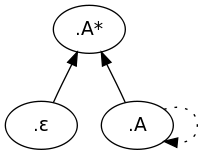
\includegraphics[scale=0.5]{star-list.png}
\caption{A graph representation of an expanded star-list; the solid arrows represent edges and the dotted arrows `next pointers' in a production.}
\end{figure}

Children of expandable nodes can be shared just like any other graph node. Since this is the case, worst-case time and space bounds do not change by the introduction of this feature.

Exactly the same principle is used for all expandables. We will not go into detail on any others, since one can easily imagine how this works.

\section{Optimizations}
\label{chap:optimizations}

The basic algorithm is fairly straightforward and relatively simple to implement. The naïve implementation will respect worst-case cubic time and space bounds, however adaptations can be made to improve its overall efficiency.

\subsection{General}

\subsubsection{Matching}
A minor performance improvement can be made by matching on entire literals at once, instead of on individual characters. This decreases the amount of necessary graph nodes and thus reduces stack activity, offsetting the performance overhead being scannerless brings along completely. Note that, to ensure correct behaviour, the level at which each literal ends is the level in which it needs to be handled.

In essence, this optimization is fairly similar to having a built-in parallel scanner.

\subsubsection{Eager matching}
As one may have noticed, in our algorithm, we do not distinguish between the handling of leaf nodes in the graph (literals, characters, epsilons, etc.) and non-leaf nodes (non-terminals, lists, optionals, etc.). Making this distinction will however open up more possibilities for optimization, as certain assumptions related to specific graph nodes can be used to handle them more efficiently.

One of these optimization we would like to call eager matching. What it boils down to is that we can prevent unnecessary work by checking whether or not a leaf node in the graph will match the input before actually constructing this node. This is an optimization that is trivial to implement, but can have a fairly big impact, as the amount of unnecessary work it prevents can be significant. This optimization can be applied to both the expansion code and the code which handles the movement to the `next' items in productions.

\subsubsection{Look-ahead}
A more obvious optimization is adding support for look-ahead filtering. By adding simple checks to the (generated) parser code, we can prevent unnecessary work; if we can determine up front that a certain alternative will never match, we do not need to expect it. This both improves performance and will make recognizing / parsing deterministic for all classes of LL grammars. When the prefix-sharing optimization (see section \ref{sec:prefixSharing}) is enabled, this will also be the case for all grammars that fall within any LR class.

\subsubsection{Breadth-first}
Finally we would like to note that (as we hinted in section \ref{sec:breadthFirstVsDepthFirst}) a breadth-first general parsing algorithm, or breadth-first implementation of a general parsing algorithm is generally more efficient then a depth-first version. The guarantee of being level synchronized can be exploited by the recognizer / parser, enabling the possibility of handling certain things more efficiently; this mainly has a positive effect on memory usage.

\subsection{Edge related}
\label{sec:edgeOptimizations}

Generally parsers store results on edges in the graph. If we would refrain from doing this and store parse results elsewhere (in a table with constant look-up time), edges could remain pointers. At first sight this may not look like an advantage, however we would be able to share edges among graph nodes and it opens up numerous other opportunities for optimization.

\subsubsection{Expansion}
\label{subsec:nodeExpansionOptimization}
First of all, by caching `expected children' for every type of node per level a substantial performance increase can be achieved. Additionally, this will ensure linear scaling relative to the size of the grammar, regardless whether or not the grammar contains (hidden) left recursive rules. The reason for this is the following; for example, if we take the grammar rules:\\
$S\,::=\,E$\\
$E\,::=\,E + E\,|\,E - E$\\
The expansion at the first level, without any optimizations, would look like this:
\begin{enumerate}
 \setlength{\itemsep}{0pt}
 \setlength{\parskip}{0pt}
 \setlength{\parsep}{0pt}
 
 \item $.E$ $\rightarrow$ $.E+E$
 \item $.E+E$ edges = \{$.E$\}
 \item $.E$ $\rightarrow$ $.E-E$
 \item $.E-E$ edges = \{$.E$\}
 \item $.E+E$ $\rightarrow$ $.E+E$
 \item $.E+E$ edges = \{$.E$, $.E+E$\}
 \item $.E+E$ $\rightarrow$ $.E-E$
 \item $.E-E$ edges = \{$.E$, $.E+E$\}
 \item $.E-E$ $\rightarrow$ $.E+E$
 \item $.E+E$ edges = \{$.E$, $.E+E$, $.E-E$\}
 \item $.E-E$ $\rightarrow$ $.E-E$
 \item $.E-E$ edges = \{$.E$, $.E+E$, $.E-E$\}
\end{enumerate}
This example clearly demonstrates quadratic behaviour. If we would cache the edges set of one $E$, we could reuse it for any other $E$ in the same level and enable us to update it with additional edges by reference. This is possible since nodes are guaranteed to have the same edges if they are `expected' by the same parent(s). This will make the expansion look like this:
\begin{enumerate}
 \setlength{\itemsep}{0pt}
 \setlength{\parskip}{0pt}
 \setlength{\parsep}{0pt}
 
 \item $.E$ $\rightarrow$ $.E\,+\,E$
 \item $.E$ $\rightarrow$ $.E\,-\,E$
 \item $E$ edges = \{$.E$\}
 \item $.E+E$ $\Rightarrow$ $E$ edges += $.E+E$
 \item $.E-E$ $\Rightarrow$ $E$ edges += $.E-E$
\end{enumerate}
Now expansion completes in linear time. An additional benefit is that all the edge sets are shared between the children of the different $E$'s, saving memory. It will cause the worst-case number of edges to scale with a factor that is equal to the number of sorts in the grammar. Originally, without this kind of sharing, this factor would have been equal to the square of the number of productions in the grammar; so this optimization results in an improvement of both a factor as an order of magnitude. One other benefit of this optimization is that it lessens the need for the left-factoring of grammars. In absence of look-ahead filtering, expansion performance should be on par with the non-factored equivalent of the grammar; in cases where look-ahead information is used, it may be close enough to remove its necessity.

Also note that this optimization is not only useful in case we have numerous non-factored productions. It also causes the set of edges to be shared between different alternatives associated with the same left-hand-side. So even if we would enable the sharing of the prefixes of alternatives (see \ref{sec:prefixSharing}), we would still gain something.

In section \ref{sec:factoringBenchmark} we look at some experimental results related to this optimization.

\subsubsection{Sharing}
Secondly, since the sets of edges, mentioned in section \ref{subsec:nodeExpansionOptimization}, are uniquely associated with a level and a certain non-terminal sort, we can reuse these sets of edges for each item in the production. When moving to the next node in a production we transfer each of the sets of edges to this next node, depending on whether or not it is already present; if a set of edges is present for a certain level in this next node, it is guaranteed to be the exact same set of edges as we are trying to add. Because of this guarantee, it will never be necessary to duplicate these sets of edges or any of their content. The result of this is that the worst-case number of edges will never exceed $N\,*\,\mathit{numberOfSorts}$, or $O(N)$, in total. If we would duplicate all the edges in the edges sets while transferring them to the next node in the production, the worst-case number of edges would both become quadratic and scale with a factor that is related to the number of items in the grammar. So this optimization, in combination with the previously outlined edge sharing optimization, results in quite a substantial improvement.

\subsubsection{Visiting}
\label{subsec:edgeVisitOptimization}
As mentioned before, since every graph node that contains the same non-terminal sort always has the same children if they are in the same level, it is sufficient to initially just follow the first edge in the edges set associated with that level. In case the node this edge points to already has registered derivations, nothing needs to be done for this node or any of the other edges in this set (except record the results for the alternative, in case we are parsing and not just recognizing); otherwise all other edges in this set need to be followed as normally would have been the case, to queue their associated nodes for reduction. This reduces the number of edge visits significantly, in certain cases, when parsing for an ambiguous grammar. Additionally, it enables us to quickly determine whether or not the parents of a node still need to be reduced, without having to execute any additional checks.

\subsubsection{Conditional edge sharing}
As mentioned earlier, distinguishing between different types of graph nodes can open up interesting opportunities for optimization.

One of these optimizations is conditional edge sharing. The guarantee that an identical collection of sets of edges on a leaf node in the graph will always be present on the `next' item in the production (if any), can be used to increase the level of edge related sharing. The reason this is true is because leaf nodes always have a static length. This property makes it impossible for a stack merge to occur on any node that is located directly after a leaf node in a production. For this reason the structure holding the sets of edges on a leaf node can be shared with its immediate right neighbour in the production. The only exception that needs to be taken into account is related to empty leaf nodes (epsilons), as sharing their sets of edges may cause interference with the hidden right recursion fix. While epsilons are not intended to be located in the middle of a production, which makes this is a non-issue in general, there are scenarios imaginable where this may be desirable and thus we need to take the possibility of this occurring into account.

\subsection{Graph}

\subsubsection{Prefix sharing}
\label{sec:prefixSharing}
In many grammars productions exist that start with the same symbol or series of symbols. There is no reason to do duplicate work for these symbols. For example, if we take the grammar rule: $S\,::=\,E\,+\,E\,|\,E\,-\,E$. Both $E$'s at the start of these productions will always be derived exactly the same way for the same substring(s) and thus they are equal. Because of this, the prefixes of these two productions may as well be merged; i.e. by converting the rule into $S\,::=\,E\,(+\,E\,|\,-\,E)$.

It is trivial to modify our algorithm to support this. Simply by allowing every node in the graph to have more then one `next' node, the desired result can be achieved. Naturally the merged prefixes of grammar rules can be arbitrarily long and are not restricted to just two partially equal rules; as long as the prefix for the rule overlaps with that of another rule, it can be merged.

This optimization ensures that, in combination with look-ahead filtering, we can recognize and parse all classes of LR grammars deterministically, since there will only be one active stack at most.

One may wonder why merging anything other then the prefixes of productions is not supported. While, in theory, sharing the postfixes of productions is also possible, this is more complicated to implement (for reasons we will not elaborate on here) and we assume that opportunities to apply this optimization rarely occur in reality. For these reasons we decided not to add this feature to our recognizer / parser. Merging blocks of symbols that are not located at either the beginning or end of productions will never be possible for our algorithm, since this may lead to incorrect results. For example if we had shared the $B$ of the following alternatives: $S\,::=\,ABC\,|\,DBE$ we would also end up with derivations for $ABE$ and $DBC$, which is obviously undesirable.

\pagebreak
\section{Filtering}
\label{chap:filtering}

As is common in general parsing, ultimately you may end up with an ambiguous parse forest. In this chapter we will discuss a number of features that can be used to filter the trees in an ambiguous parse forest, in case this is required. These features are all optional and have no dependencies on each other.

\subsection{Restrictions and requirements}

First of all one could add restrictions to grammar items. For example, in case one wants to indicate eagerness for a certain item, one could mark this item with a restriction that prevents it from being followed by a specific set of characters or strings. Another example would be a restriction which specifies that a certain item should always start at the beginning of a line, or a specific column. One can think of numerous different possibilities; basically any restriction or requirement on the substring an item matched or the input preceding or following an item is imaginable.

When adding this feature to the implementation of the recognizer / parser one can make the distinction between filters that need to be executed before reduction and filters that can also be executed before the expansion of an item, for efficiency reasons. Filters that can be executed before the expansion of an item are almost exclusively limited to restrictions and requirements that deal with input that precedes an item, all other filters can only be handled before the reduction of their associated item, since we generally do not have all the required information to handle these before that time. When a filter successfully matches, it prevents either the expansion or reduction of the item it is associated with, both to prohibit the recognizer from recognizing it and preventing the possible results this item would have had from being added to the parse forest.

\subsection{Nesting restrictions}

Another disambiguation feature we supply comes in the form of nesting restrictions. These restrictions can be used to indicate that certain reduction paths are invalid. This enables us to, for example, support things such as priority and associativity rules in grammars.

If one would like to implement priority and associativity rule handling, this would go as follows. If we take the grammar rule $E\,::=\,E\,*\,E\,>\,E\,+\,E$, where the $>$ sign indicates that $E\,*\,E$ has a higher priority then $E\,+\,E$, this would mean that $E\,+\,E$ cannot be nested on either side of the $E\,*\,E$ alternative, since $E\,*\,E$ binds stronger. Associativity rule handling works in a similar way. If the rule $E\,::=\,E\,+\,E$ would be declared as being left associative, this means that it is not allowed for $E\,+\,E$ to be a child of itself at the rightmost $E$ of this alternative. Right or non-associativity can be achieved similarly. This restriction scheme allows priorities and associativity to both be mixed and nested arbitrarily.

Our current implementation handles nesting restriction filtering completely at parse time. While reducing it checks whether or not each of the reductions are allowed; in case it is (and we are parsing), the result is stored in a result node that is identified by the sort name of the non-terminal which the edge we are currently following points to and the set of nesting restrictions associated with this node. This is because the result needs to be shared between all the items associated with the same non-terminal sort and set of nesting restrictions. The reason for this sharing is twofold. First of all it is required to enable the parser to handle cycles involving rules containing nesting restrictions correctly (in case they occur). And secondly, for the sake of efficiency.

The main advantage of handling nesting restrictions at parse time, opposed to implementing it as post-parse filter, is that it is more efficient. We prevent the construction of results that will be discarded later on, saving memory. Additionally it will prevent unnecessarily exploring certain parses, because we can determine they will be filtered earlier on, decreasing the total amount of work that needs to be done. For certain grammars the benefits of this approach can be very significant. Furthermore, it also enables the possibility of constructing a recognizer for languages that require nesting restrictions for disambiguation. This is because the way the filtering is implemented does not require any results to be constructed, rather it just prevents certain stacks from progressing.

There is however one additional thing that needs to be noted. Handling nesting restriction filtering at parse time, in the way described, disables the edge visit reduction optimization discussed in section \ref{subsec:edgeVisitOptimization}, since we now always need to visit each of the outgoing edges of a node at every reduction to check whether or not the nesting is allowed. Fortunately, this only potentially impacts performance in case the production we are handling is ambiguous. Additionally, it is reasonably simple to detect whether or not any nesting restrictions need to be applied for each batch of reductions. So it is possible to dynamically determine the appropriate reduction code path, depending on the type of node that needs to be handled. This means any possible performance impact remains limited to the handling of rules on which nesting restrictions apply.

One last thing that needs mentioning is that the handling of nesting restriction can be implemented in a even more efficient way, as we currently determine whether or not a nesting is allowed after we have recognized the alternative. It is possible to prevent any unnecessary work from being done by executing the filtering at an earlier stage in the parse process. This would involve pre-computing allowed nestings and clustering alternatives or continuations of alternatives with similar nesting restrictions. Each of these clusters could then either be expanded or not for a certain item. This would allow the parser to become more deterministic on grammars containing nesting restrictions, improving scalability and performance at the potential cost of an increased amount of items, as the clustering could possibly prevent certain prefixes of alternatives, either partially or wholly, from being shared. The impact of this optimization can be very significant in some cases (e.g. it can potentially change the worst-case upper bound of certain grammars from cubic to linear); on the other hand this optimization can be reasonably complex to implement.

\subsection{Semantic actions}

Support for semantic actions is also present. Each grammar rule can have a number of semantic actions associated with it. These semantic actions can be used to filter ambiguities that cannot be disambiguated using other filters, including non-context-free ambiguities (like C typedefs). It even opens up the opportunity to influence the behaviour of the parser while it is running.

One has the choice to, either partially or wholly, integrate the execution of semantic actions into the core of the parser itself or to apply them as a post-parse filter during, or after, flattening; depending on the requirements or preference of the user. Keep in mind that the implementation of semantic action support is not trivial, both because of their interaction with ambiguities and the parse forest and the possible side-effects they can have. Depending on what types of actions one wants to support, integrating them into the parse process itself can be especially challenging. Postponing the execution of actions until after the parsing and flattening process, when we are in possession of a complete parse forest, is by far the easiest alternative, but also the least optimial.

We will not go into detail about the implementation of actions, since that is outside the scope of this article. However, we will outline a proposal about how one could accommodate the integration of actions, to give an impression of what is involved and what issues may arise when implementing an alternative solution.

\subsubsection{Intergration}
The framework we propose for handling the execution of actions is fairly involved. Mostly, because we need to be able to handle actions with side-effects on different branches of ambiguous trees and support the ability to backtrack and merge environments. Both to make everyone's life slightly easier and to make it simpler for users to redefine the way actions are handled (if needed), we propose to integrate the handling of actions in the flattener, instead of the core of the parser itself. While we lose the ability to influence the parser while it is running (which is a relatively scary thought anyway), we still remain fairly efficient. Postponing the execution of actions until after the completion of the flattener would simplify things further, but would also require a second pass over the parse forest and it has several other drawbacks which make it less desirable performance wise. Another consideration discouraging the integration of the handling of semantic actions in the parse process itself was that it would cause the parser to exceed its worst-case time and space bound guarantees, since each result needs to be flattened before one can invoke any action on it. This is an additional reason why the integration of the execution of semantic actions in the flattener is a better fit. A hybrid solution is also imaginable, where only certain types of actions are allowed to be executed during the parse process and all others are handled afterwards.

As mentioned, it is possible for actions to have side-effects. Most of the complications related to actions stem from this property. In cases where there is more then one alternative parse result for a certain part of the tree, the side-effects of actions on one alternative should not have an impact on actions on any of the other alternatives, including their sub trees. To facilitate this we introduce the concept of environments, which can be linked together to form a stack. While traversing the parse forest we fire events, each of these events requests a response from the action executor. For example, if we are about to flatten a production which has an action associated with it, the event indicating that this is the case enables the user to push a new environment on the stack, if required. The popping of environments, on the other hand, should be handled by the flattener itself; although all the events that would be required by the user to handle this themselves should be fired regardless, so users are able to maintain their own shadow hierarchy of environments if necessary.

Basically, there are three types of events; either we enter or we exit something or we need to apply an action to a certain tree construct. If we receive an enter event, we have the opportunity to prepare everything for the handling of the indicated construct, like pushing a new environment on the stack. If we receive an exit event, we should be notified whether or not the construct we are handling was successfully build or got filtered; so any bookkeeping actions can be executed, if required. Finally, we have the filter events, which request the execution of any with the indicated construct associated semantic actions. These constructs can either be alternatives for productions, ambiguity clusters or cycles. Each action has the opportunity to either replace the given construct by an alternative version or have an arbitrary side-effect on any of the environments on its associated stack.

Something else to keep in mind is how the sharing of the results is handled. Because of the potential side-effects that actions can have, one cannot determine whether or not a certain previously constructed result can be reused as easily. Generally this is only the case when the construct we are handling and all of its potential direct and indirect children are side-effect free and do not rely on side-effects themselves. In all other cases the result will need to be reconstructed; unless the content of the current environment is equal to one which is associated with any of the previously constructed results for the construct we are currently handling.

\section{Benchmarks}

In this chapter we will have a look at the performance of the current Java implementation of our algorithm.

Benchmarks were executed on a machine with the following specifications:
\begin{table}[H]
\centering
\begin{tabular}{ | p{6em} | p{9em} | }
 \hline
 CPU & Intel Q6600 \\
 Memory & 8 GB DDR-800 \\
 OS & Fedora Core 12 \\
 JRE & Sun 1.6.0\_13 (32-bit) \\
 JRE options & -Xmx1800m \\
 \hline
\end{tabular}
\end{table}

Measurements are listed in terms of CPU-time (system + user time) and are gathered using Java's build in management tool. Before performing the benchmarks, the recognizer / parser code was executed a number of times so Java's JIT compiler has the opportunity to optimize.

\pagebreak
\subsection{Worst case}
\label{sec:worstcaseBench}

The obvious candidates for a benchmark are the following worst-case grammars:
$S\,::=\,SSS\,|\,SS\,|\,a$\\
And:\\
$S\,::=\,SSS\,|\,SS\,|\,a\,|\,\epsilon$\\
With as input:\\
$a\,*\,50$ to $a\,*\,500$ at $50$ character intervals.

\begin{figure}[H]
\centering
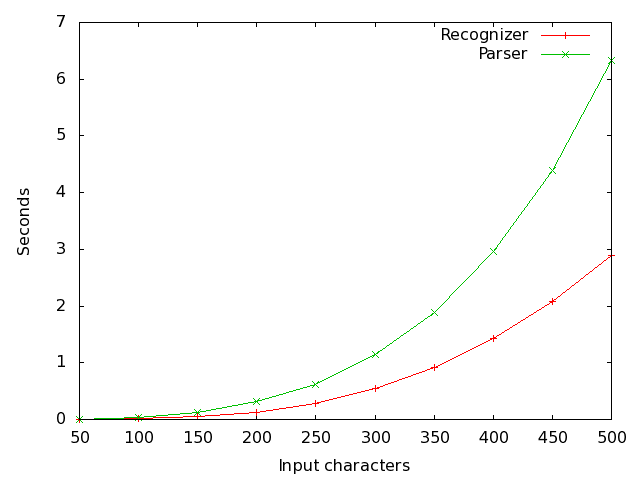
\includegraphics[scale=0.4]{worst-case.png}
\caption{$S\,::=\,SSS\,|\,SS\,|\,a$ recognizer and parser performance scaling.}
\end{figure}

\begin{figure}[H]
\centering
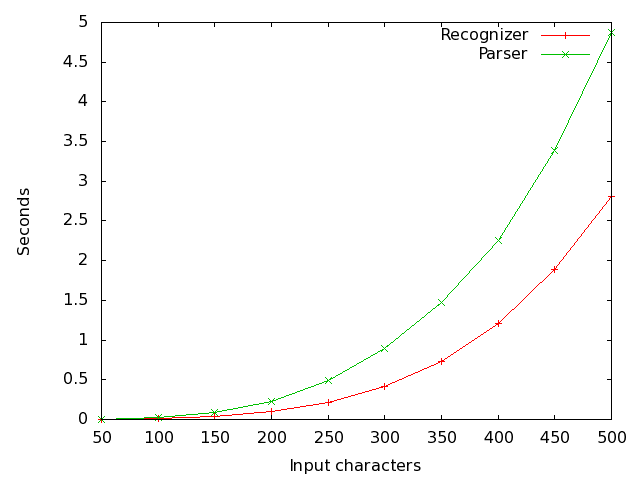
\includegraphics[scale=0.4]{worst-case_with-epsilon.png}
\caption{$S\,::=\,SSS\,|\,SS\,|\,a\,|\,\epsilon$ recognizer and parser performance scaling.}
\end{figure}

Our recognizer and parser implementations clearly demonstrate cubic worst-case behaviour, as expected. Looking at the times, our implementation seems very efficient in worst-case scenarios.

Note however that the recognizer is optimized for speed and the parser for a balance between memory usage and speed (meaning a faster implementation is possible at the cost of an increased memory footprint).

What may appear surprising to some is the limited performance difference between both cases. Even though the version which includes the $\epsilon$ yields a more complicated tree and nullables need some special care, the actual extra work involved in handling them is negligible. This is in line with what we asserted in section \ref{subsec:hiddenRightRecursion}.

\subsection{Grammar factoring}
\label{sec:factoringBenchmark}

Apart from worst-case behaviour in terms of the number of ambiguous parse results, it is also interesting to look at how well we perform on a different kind of worst-case scenario, without ambiguous input. Here we will compare the performance of our parser between different versions of an expression grammar; a non-prefix-shared version, a prefix-shared version and an equivalent left-factored version. The only purpose of this test if to highlight the effects of grammar factoring on the performance of the expansion phase in the parser. The original grammar is the following:\\
$S\,::=\,E+$\\
$E\,::=\,a\,|\,E\,+\,E\,|\,E\,-\,E\,|\,E\,*\,E\,|\,E\,/\,E\,|\,E\,>\,E\,|\,...$ 25 more like it ...\\
Input = $a\,*\,50000$, $a\,*\,100000$, $a\,*\,150000$ and $a\,*\,200000$

This grammar contains a lot of recursion and is highly ambiguous; the input, on the other hand, can not be parsed in more then one way. Regardless, one might expect non-linear performance when parsing a string for this grammar with a top-down parser. However, as can be seen in the graph below, this is not the case for our algorithm. In this benchmark, performance scales perfectly linear regardless of how the grammar is factored.

\begin{figure}[H]
\centering
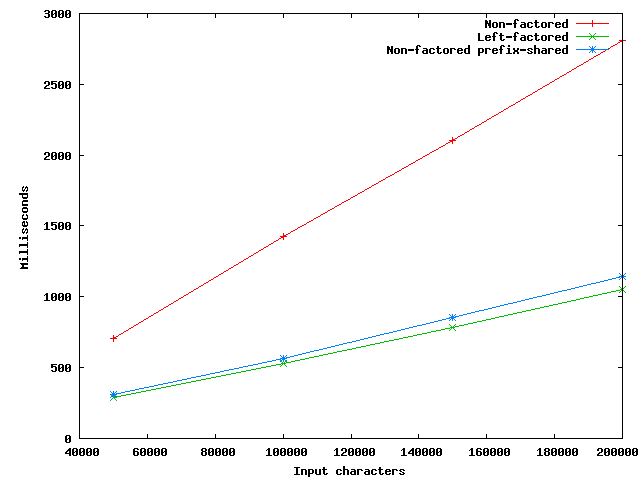
\includegraphics[scale=0.4]{grammar-factoring.png}
\caption{Grammar factoring related parse time scaling.}
\end{figure}

Our parser is more then four times as fast on the non-factored version of the grammar when prefix sharing is enabled. This is because both the number of graph nodes as the number of edge visits is significantly higher in case it is disabled. However, parsing performance still scales linear with respect to the length of the input regardless of this, due to the expansion optimization discussed in section \ref{subsec:nodeExpansionOptimization}.

As can be seen, the non-factored prefix-shared and the left-factored versions of the grammar are fairly close together in terms of performance. The reason why our parser performs slightly better on the prefix-shared version of the grammar in comparison to the left-factored version, is purely a result of the transformation that was required to achieve the left-factoring.

Surprising though is that, while this benchmark is one of the cases that is most heavily biased in favor of look-ahead filtering, the impact it has is hardly noticeable. Look-ahead filtering should have a positive influence on performance while parsing a string for the left-factored version of the grammar, however the impact it has is so minor that it is hardly measurable. The main reason for this is the eager matching optimization, achieves almost the same effect as look-ahead filtering would have in this particular case. However, there are other situations in which look-ahead filtering can still be a potentially useful performance enhancing tool.

One other thing to mention is that the left-factoring of the grammar also removes all ambiguities from it. Contrary to what one might expect, this does not have an impact on performance in this specific case, since in both the prefix-shared as the left-factored case there will never have more then one live stack.

\subsection{Versus non-general}

We also liked to know how we compare when pinned against non-general parsers, since general parsers have the image of being inferior in terms of performance, in relation to non-general LL or (LA)LR parsers.

We used the following basic LR grammar for our benchmark:\\
$S ::= E$\\
$E ::= E + F\,|\,F$\\
$F ::= a\,|\,(\,E\,)$\\
Input = `$A\,::=\,a\,|\,a+(A)$' from length $100003$, to length $1000003$ at $200000$ character intervals.

We compared our performance with JavaCup\cite{javacup} (which was used in combination with JFlex\cite{jflex}), SGLR\cite{sglr}, JSGLR\cite{jsglr} and Bison\cite{bison} (in combination with Flex\cite{flex}). We selected JavaCup, since it is one of the more widely known and used parser generators that produces LALR parsers in Java. SGLR, on the other hand, is a general parser (written in C) which we extensively used in the past. The reason we included JSGLR is to enable a better comparison against our own, since it is similar to SGLR but also written in Java. Finally, Bison was selected to complete the picture, as it is one of the most widely known LALR parsers.

To make the comparison as fair as possible, all parsers were purely executed as recognizers, so no trees were build and no filtering was applied. Both SGLR and Bison were compiled using GCC 4.2.2 with `-O2'. Additionally, we disabled the GSS garbage collector for the C implementation of SGLR, to enable a fair comparison, since it was triggering quadratic behaviour.

\begin{figure}[H]
\centering
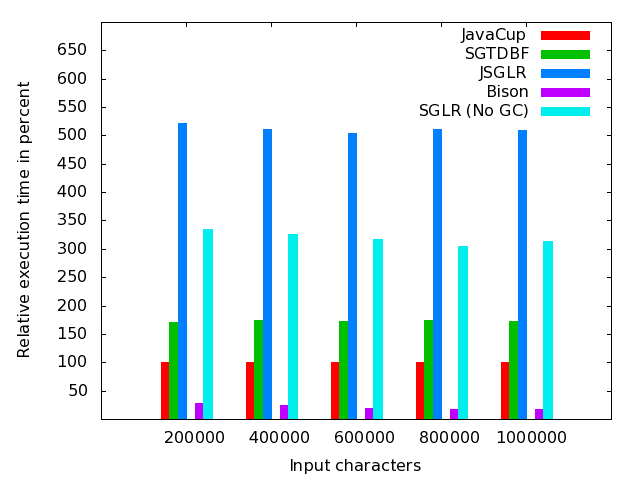
\includegraphics[scale=0.4]{vsLALR.png}
\caption{A parsing performance comparison between different parsers.}
\end{figure}

As expected JavaCup performs best in the Java category. For this specific grammar, the JavaCup parser consistently recognizes the given input between one and a half and two times as fast as our parser. This seems like a big difference, however this is a fairly impressive result. Especially, since our parser interprets the grammar at runtime, whereas JavaCup generates directly executable parser code. Additionally, one also needs to consider that we are using a graph to model the stack, since we need to be fully general, instead of using the application's stack. When looking at the results for JSGLR it becomes even more apparent how well we do in comparison.

In the C category Bison dominates. SGLR is over fifteen times slower then Bison on this grammar. As can be seen, our parser also outperforms SGLR by quite a significant amount.

Apart from this, our parser scales perfectly linear for this grammar, like the others. The data in the graph supports this, as the relative performance difference between the parsers does not change for increasing input lengths.

It is worth mentioning that it is still possible to further optimize the performance of our parser on LL and (LA)LR grammars. One could imagine implementing a faster path for productions in slices of the grammar that conform to certain restrictions (i.e. they only contain non-terminals that are in LR(k) for example). By doing this we would be able to match the speed of any competing parser.

One also has to take into account that, while our parser handles itself nicely in this benchmark, when compared to other in Java written parsers, an equivalent C implementation would perform much better.

\section{Prototype}

The development of this algorithm was approached in a rather unorthodox way. Rather then starting with the design of the algorithm and making an implementation for validation and testing purposes afterwards, we started with implementing a basic top-down recognizer, extending it to a parser, followed by testing, profiling and optimization; gradually we improved this implementation and its algorithm, until it matched our requirements. By using this type of approach we were able to get more direct feedback about issues and scalability and performance bottlenecks. Additionally, opportunities for optimization were highlighted that may not have been immediately apparent or which may have been overlooked when the problem would have been approached from a purely algorithmic point of view.

The main purpose of this project has always been to create a working, usable general context-free parser implementation. The development of a new algorithm was secondary but required, since no suitable alternative was available for our purposes.

Our first implementation is written in Java. The reason we chose this language for our prototype was that is was both required for our current project (the interpreter and IDE for the Rascal\cite{klint2011easy} meta programming language), and gave us the opportunity to easily change and extend it. The down side is that it makes it harder to make a comparison with other (general) parser implementations, which are mainly written in C and consequently have a major performance advantage.

\section{Future work}

Numerous things can still be improved or changed. Mostly these involve optimizations or implementation improvements. We will not go into detail, but just list a number of ideas instead.

\begin{itemize}
 \setlength{\itemsep}{0pt}
 \setlength{\parskip}{0pt}
 \setlength{\parsep}{0pt}
 
 \item We can pre-construct a data structure which contains mappings from non-terminal sorts to alternatives; optionally in combination with their associated look-ahead information. This can aid in increasing the performance of the expansion phase.
 \item Pre-computed information about nesting restrictions can be used to improve scalability and performance.
 \item Multi-core / processor support is relatively easy to add and may be interesting to explore as possible performance booster for certain cases.
 \item The ability to generate directly executable parser code may be an interesting feature to look in to. This would further increase performance and open up new opportunities for optimization.
 \item Implement a faster path for handling productions in grammar slices that conform to certain restrictions (for example, if they only contain non-terminals that are in LR(k)), to improve performance on non-ambiguous grammars even further.
\end{itemize}

Finally, it would be interesting to create a C implementation of our parsing algorithm, both to see how far we can push the throughput of the parser and to be able to make a broader and more accurate performance comparison with implementations of other (general) parsing algorithms. We expect to do fairly well in such a showdown.

\section{Conclusion}

In this article we described our parsing algorithm, discussed optimizations that can be applied to it and gave an impression of its capabilities. To summarize, we developed a general parsing algorithm that is both easy to comprehend and scales and performs well, regardless of the input or grammar used. The world of general parsing is now one viable alternative richer.

\bibliographystyle{ieeetr}
\bibliography{bibs.bib}

\end{document}
